\chapter{Introduction}\label{chapter:intro}
The way of transportation is currently evolving and autonomous driving technology is expected to have a big impact on this transofrmation. Over one million people are killed in traffic-related accidents each year, where the vast majority of the accidents are caused by human mistakes~\cite{WHO2018, NHTSA2018}. By helping humans with perception, prediction and decision making autonomous driving could significantly improve traffic safety and make way for new innovative road infrastructure. Without the requiement of a present human for each transpotation vehicle, the efficiency of traffic can be improved by scheduling commercial transports outside of rush hours~\cite{FAGNANT2015167}.

\todo{cite future of mixed-autonomy}
% https://www.cmu.edu/traffic21/research-and-policy-papers/traffic21_policymaker_guide_summer_2021-22.pdf

\todo{level 2: volvo pilot assist and tesla auto pilot. Level 4: Waymo. Woven automated city}

Thanks to the rapid success of deep learning during the last decades, major progress towards deploying autonomous vehicles in the real world.
\tommy{rewrite}
Major progress towards deploying autonomous vehicles has been made during the last decade. The perception systems have been remarkably improved, largely due to the success of deep learning techniques~\cite{Janai2020}. The low-level control of the vehicle is a mature research area and can be solved with classical control theory methods~\cite{Paden2016}. However, how to approach the high-level decision-making in complex traffic situations is less explored and forms the main topic of this thesis.

\section{Problem formulation}

\begin{enumerate}
	\item We want to drive through intersections. 
	\item The intersection can be of different shapes. We assume we have a map of the intersection. 
	\item There will be other cars crossing the same intersection. 
	
\end{enumerate}

The work presented in this thesis investigate the following research questions:
\begin{enumerate}
	\item[\textbf{Q1.}] How can RL be used to create a decision-making agent for autonomous driving, that can handle different intersection and roundabouts (complex urban scenarios)? Learn a scalable policy that is able to handle different scenarios. relative coordinate system. Action space. 
	(specificera for att komma undan varfor har du inte kollat pa andra metoder. How can we use RL for AD )
	\item[\textbf{Q2.}] How can AD domain knowlage (and models) be used to improve the action and state space for a RL agent? MPC for actions, Particle filter for intention distrubution. How can AD domain knowlage be used to create a state and action space that improves the RL agent?
	\item[\textbf{Q3.}] How can the quality of a RL agent be imporved by accounting for uncertainty?
	(How can the uncertainty of the RL agent be utilized?) (RPF-in the output and PF-in the input space)
\end{enumerate}

\section{System architecture}
\label{sec:system_architecture}
outline system architecture and limit this papre to comfortable decisions \gls{rl}
\tommy{depending on size of chapoter consider moving it to its own chapter}
\begin{figure}[t]
	\centering
	\mbox{\parbox{\textwidth}{
			\centering
			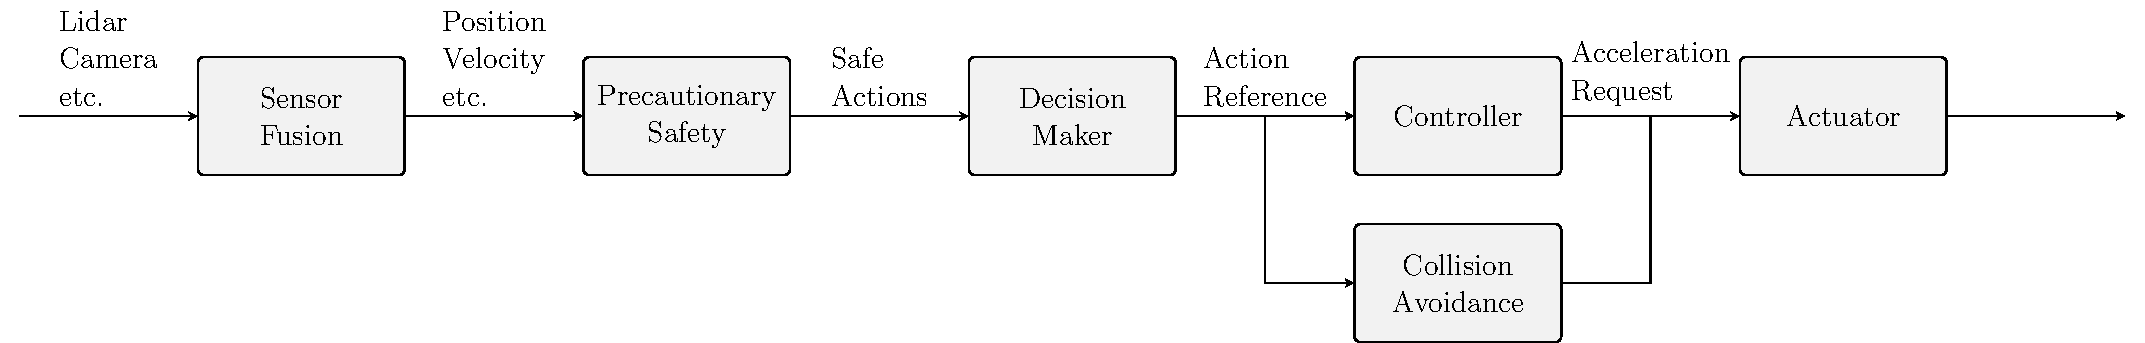
\includegraphics[width=\linewidth]{YourThesis/chapters/figures/pomdp/figures-system_architecture.pdf}%We suggest that you use a text box to insert a graphic (which is ideally a 300 dpi TIFF or EPS file, with all fonts embedded) because, in an document, this method is somewhat more stable than directly inserting a picture.   
	}}
	\caption{Representation of the system architecture.
	}
	\label{fig:system_architecture}
\end{figure}

\section{Scope and limitations}
FILL
\begin{enumerate}
	\item We have access to sensors on-board the ego vehicle. 
	\item We do not assume any knowlage of traffic signs or traffic lights. 
	\item We do not have v2v, or v2x communication. 
	\item Do not garantee safety, the best we can do its maing the decisons not trigger collision avoidance functions. 
	
	To compensate for not having v2v or v2x communitaion, we have to predict what other driver will do. 
	
\end{enumerate}


\section{Contributions}
\todo{reweite once theis is in a better state}
The main contributions of this thesis are:
\begin{enumerate}
	\item General approach to creating a decision making agent for driving in interactions. 
	\item A neural network architecture that is invariat to permutations of the order of which surrounding traffic participants are observed, which speeds up training and improves the quality of the trained agent. 
	\item A belief state representation using a particle filter and a comparison and analysis of different algorithms that ultilize the belief state. 
	\item Two approached to solving a POMDP with hidden intention state. LSTM layer and belief state. 
	\item General state space represenation that is invariat to permutations of the intersection design. 
	\item Extention of RL methods that provide an estimate of the epostemic uncertainty and use it to create a confidence critiera that can identify situations with high uncertainty. 

\end{enumerate}


\section{Thesis outline}
FILL


